\section[Example: Monte Carlo Estimation of pi]{Example: Monte Carlo Estimation of π}
\begin{frame}{Monte Carlo Method - Estimating $\pi$}
  The Monte Carlo method \parencite{Metropolis01091949} estimates $\pi$ by simulating random points in a unit square and counting how many fall inside a quarter circle of radius 1. The ratio of points inside the circle to the total points, multiplied by 4, approximates $\pi$ \parencite{beckmann1971history}.
\end{frame}



\begin{frame}{Monte Carlo Algorithm}
  \begin{enumerate}
    \item Generate $N$ random points $(x, y)$ where $0 \leq x \leq 1$ and $0 \leq y \leq 1$.
    \item For each point, check if it lies inside the quarter circle: $x^2 + y^2 \leq 1$.
    \item Count the number of points $M$ that satisfy the condition.
    \item Estimate $\pi$ as: $\pi \approx 4 \times \frac{M}{N}$ \parencite{hammersley1964monte}.
  \end{enumerate}
\end{frame}

\begin{frame}{Visual Illustration}
  \begin{center}
    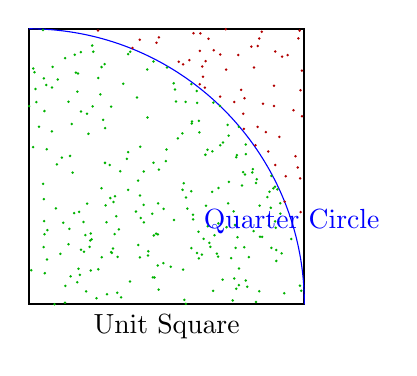
\begin{tikzpicture}[scale=3.5]
      % Draw square and quarter circle
      \draw[thick] (0,0) rectangle (1,1);
      \draw[thin, blue] (0,1) arc (90:0:1);

      \foreach \i in {1,...,300} {
          \pgfmathsetmacro{\x}{rnd}
          \pgfmathsetmacro{\y}{rnd}
          \pgfmathsetmacro{\r}{\x*\x + \y*\y}

          \ifdim\r pt<1pt
            \fill[green!70!black] (\x,\y) circle (0.005);
          \else
            \fill[red!70!black] (\x,\y) circle (0.005);
          \fi
        }

      % Labels
      \node[anchor=north] at (0.5,0) {Unit Square};
      \node[blue, anchor=west] at (0.6,0.3) {Quarter Circle};
    \end{tikzpicture}
  \end{center}
\end{frame}


\begin{frame}{Example Calculation}
  \begin{itemize}
    \item Suppose we generate $N = 1000$ random points in the unit square
    \item After simulation, we count $M = 785$ points inside the quarter circle
    \item We estimate $\pi$ as:
          \[ \pi \approx 4 \times \frac{M}{N} = 4 \times \frac{785}{1000} = 3.14 \]
    \item The true value of $\pi$ is approximately $3.14159$ \parencite{beckmann1971history}
  \end{itemize}
\end{frame}

\begin{frame}{Convergence and Error Analysis}
  \begin{itemize}
    \item The error in our estimate decreases as $O(1/\sqrt{N})$ \parencite{kalos2008monte}
    \item This means:
          \begin{itemize}
            \item $N=100$ points gives roughly 10\% error
            \item $N=10,000$ points gives roughly 1\% error
            \item $N=1,000,000$ points gives roughly 0.1\% error
          \end{itemize}
    \item The Monte Carlo method is especially useful for calculating multidimensional integrals \parencite{MonteCarloCookson2005}
    \item For $\pi$ calculation, there are more efficient methods, but this one is visually intuitive
  \end{itemize}
\end{frame}

\begin{frame}{Demo Visualization}
  \begin{center}
    \includegraphics[width=0.4\textwidth]{./programs/pi_calculation/pi_calculation.png}

    \vspace{0.5cm}
    \href{./programs/pi_calculation/pi_calculation.html}{Open Interactive Demo}
    \end{center}
\end{frame}
